% The original template (from Trevor) had a custom \appendix command,
% but I found it to break figure/table counters. I'm not sure how
% reliable my fix is, so I ended up reverting back to the standard
% latex version, and renaming the custom command to \myappendix.  You
% can try both and see how things work out:
% 1) Call \appendix once, and then make each appendix a \chapter
% 2) Call \myappendix once, and then make each appendix a \section.

\appendix

% The following affect tocloft
%\renewcommand{\thechapter}{Appendix \Alph{chapter}:}
%\addtocontents{toc}{\setlength{\cftchapnumwidth}{7em}}

\chapter{\textit{On the Use and Interpretation of Otto-Glyphs}}

    % Appendix sections, subsections etc should not appear in the table of 
    % contents. So set tocdepth to 0 and set it back to 2 at the end. Do 
    % this for each appendix.
    \addtocontents{toc}{\protect\setcounter{tocdepth}{0}}

    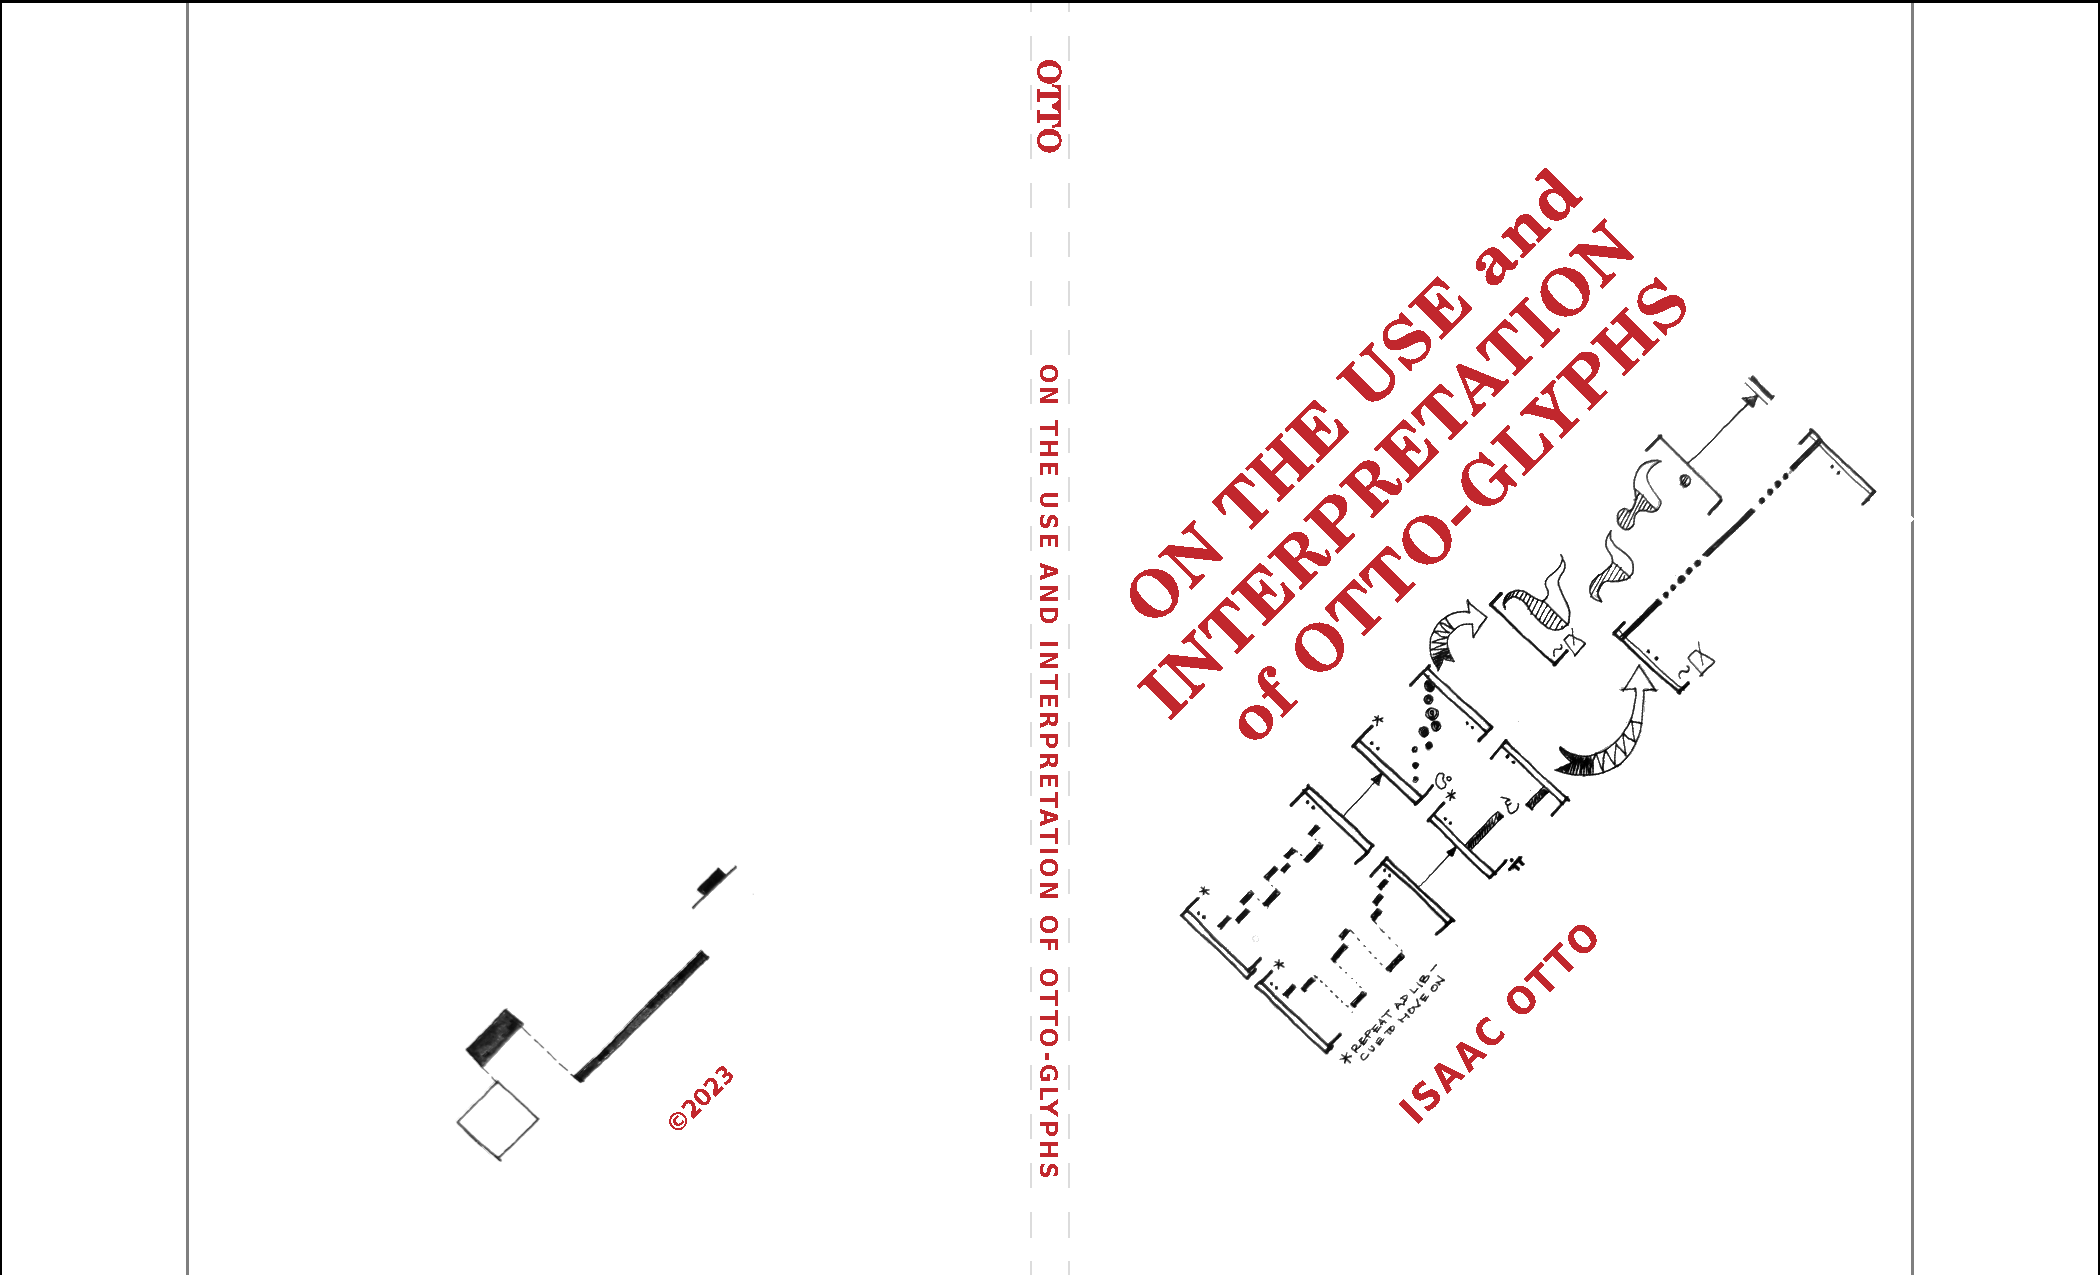
\includepdf[
        pagecommand={\thispagestyle{plain}},
        pages=-,
        frame,
        angle=270,
        scale=0.85]
    {appendix_files/instruction-cover.pdf}
    
    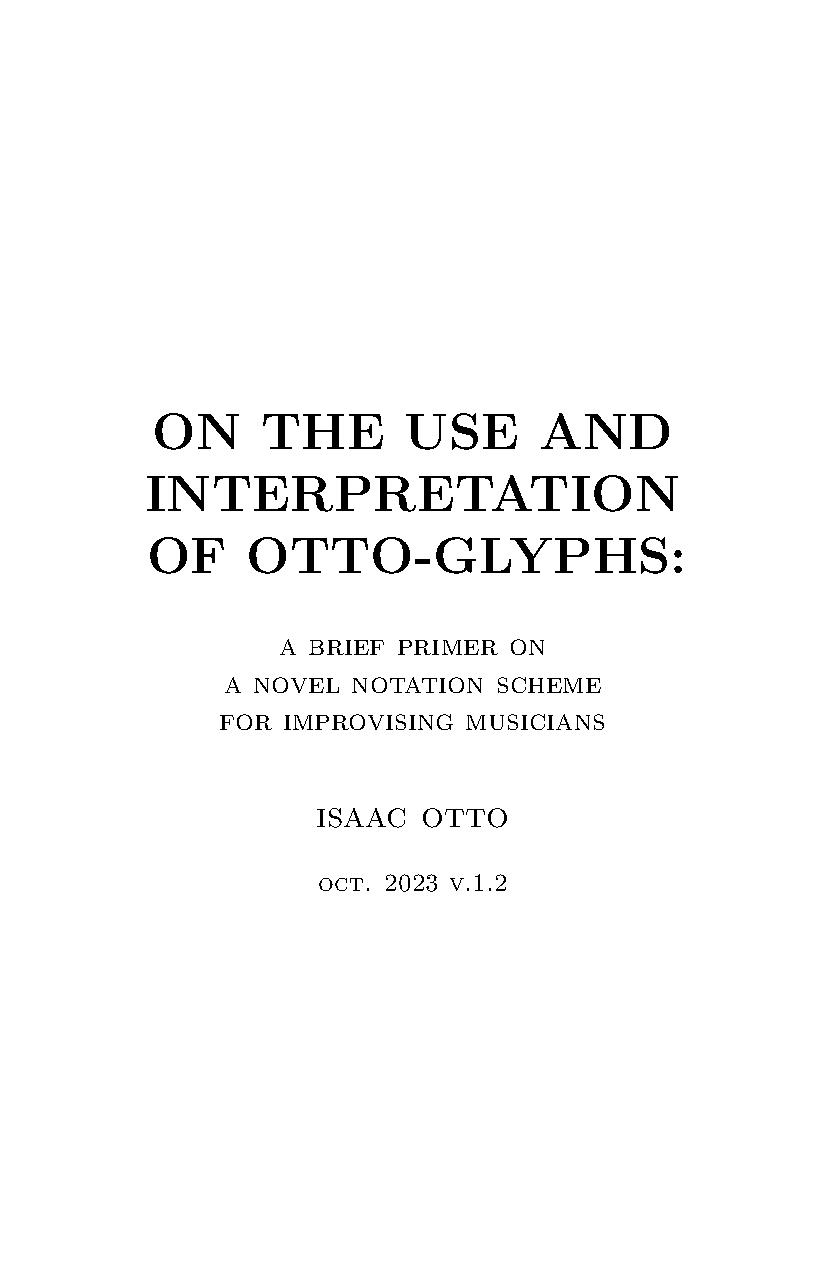
\includepdf[
        pagecommand={\thispagestyle{plain}},
        pages={1-52},
        frame,
        nup=1x2,
        angle=270,
        scale=0.85]
    {appendix_files/INST_MANUAL_INCLUDE.pdf}
    
    \addtocontents{toc}{\protect\setcounter{tocdepth}{2}}

\chapter{Program and performers' notes for \textit{I Die Each Time I Hear the Sound}}
    \addtocontents{toc}{\protect\setcounter{tocdepth}{0}}
    
        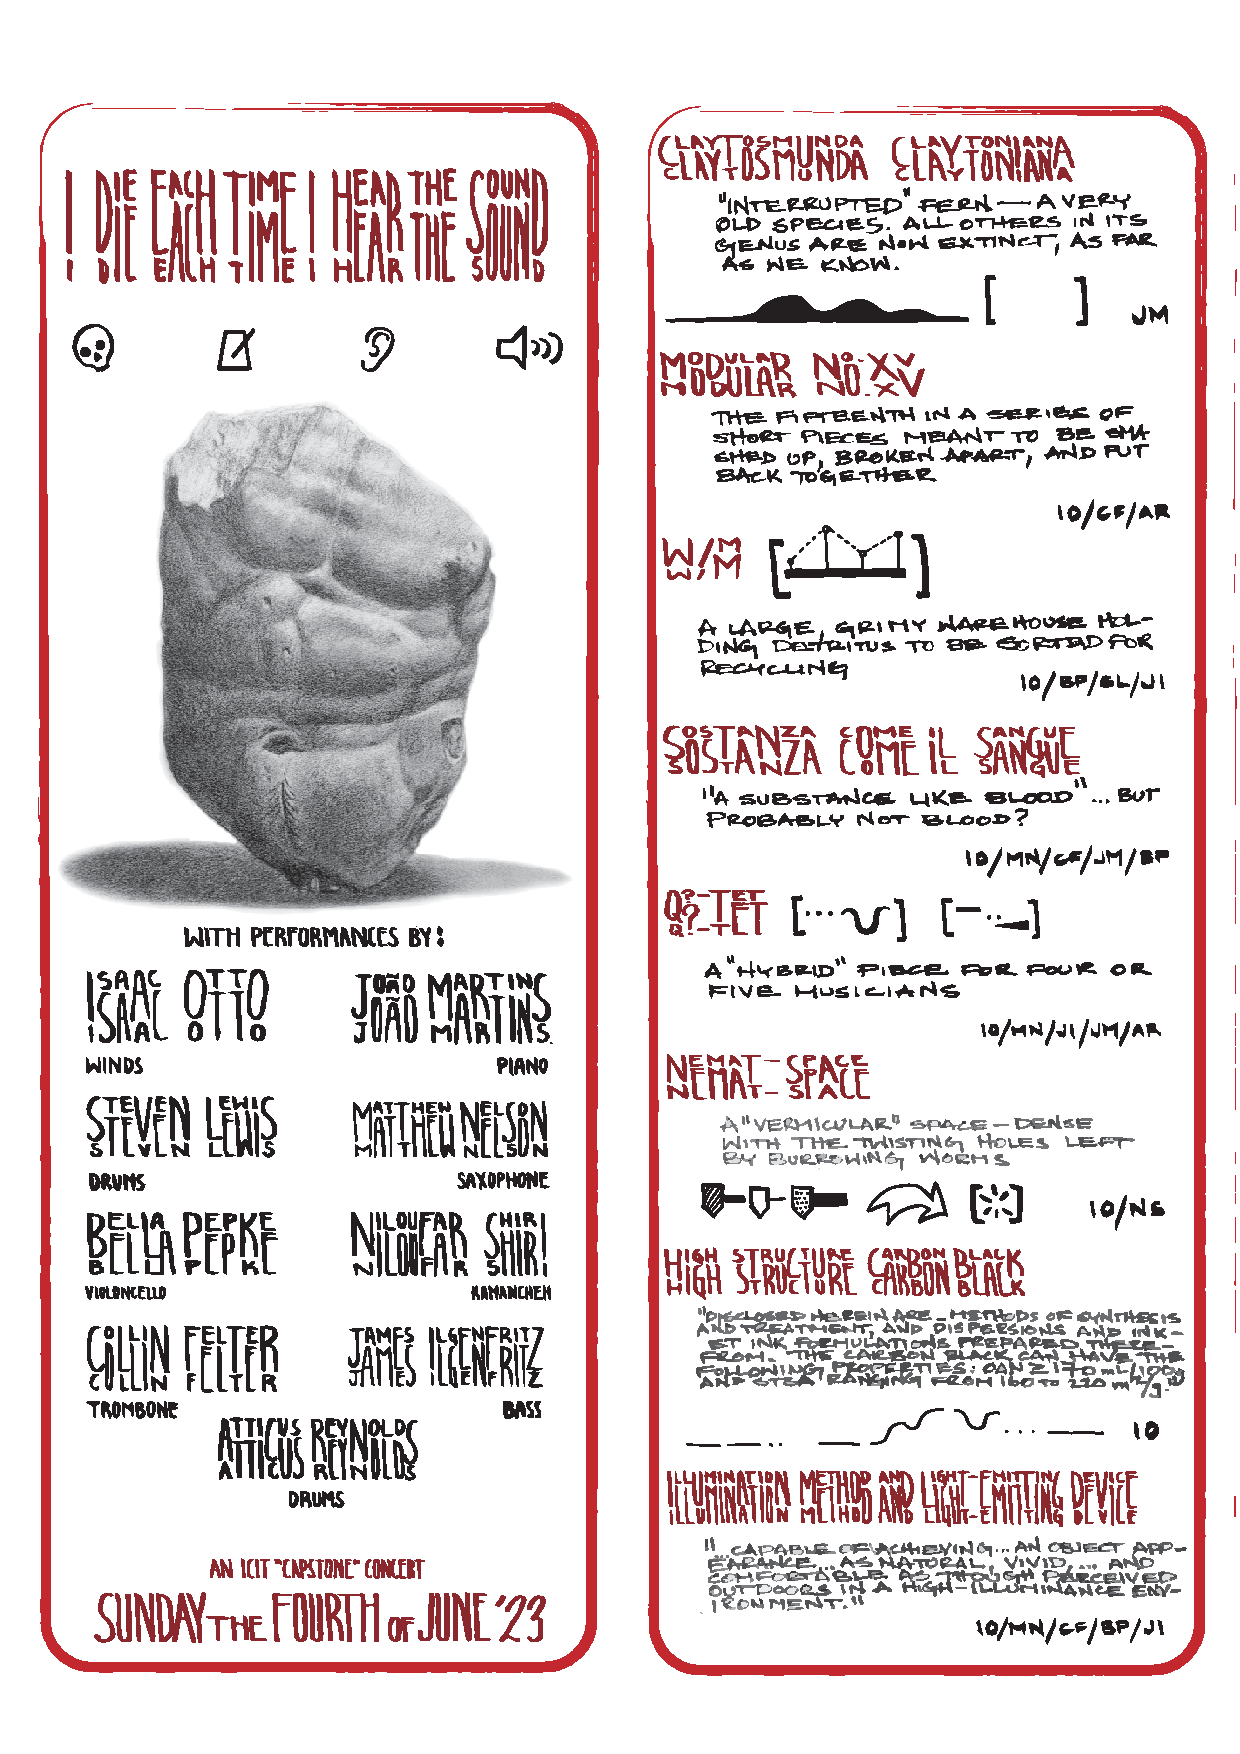
\includepdf[
            pagecommand={\thispagestyle{plain}},
            pages={1},
            frame,
            scale=0.85]{appendix_files/program_notes_front_and_back.pdf}

        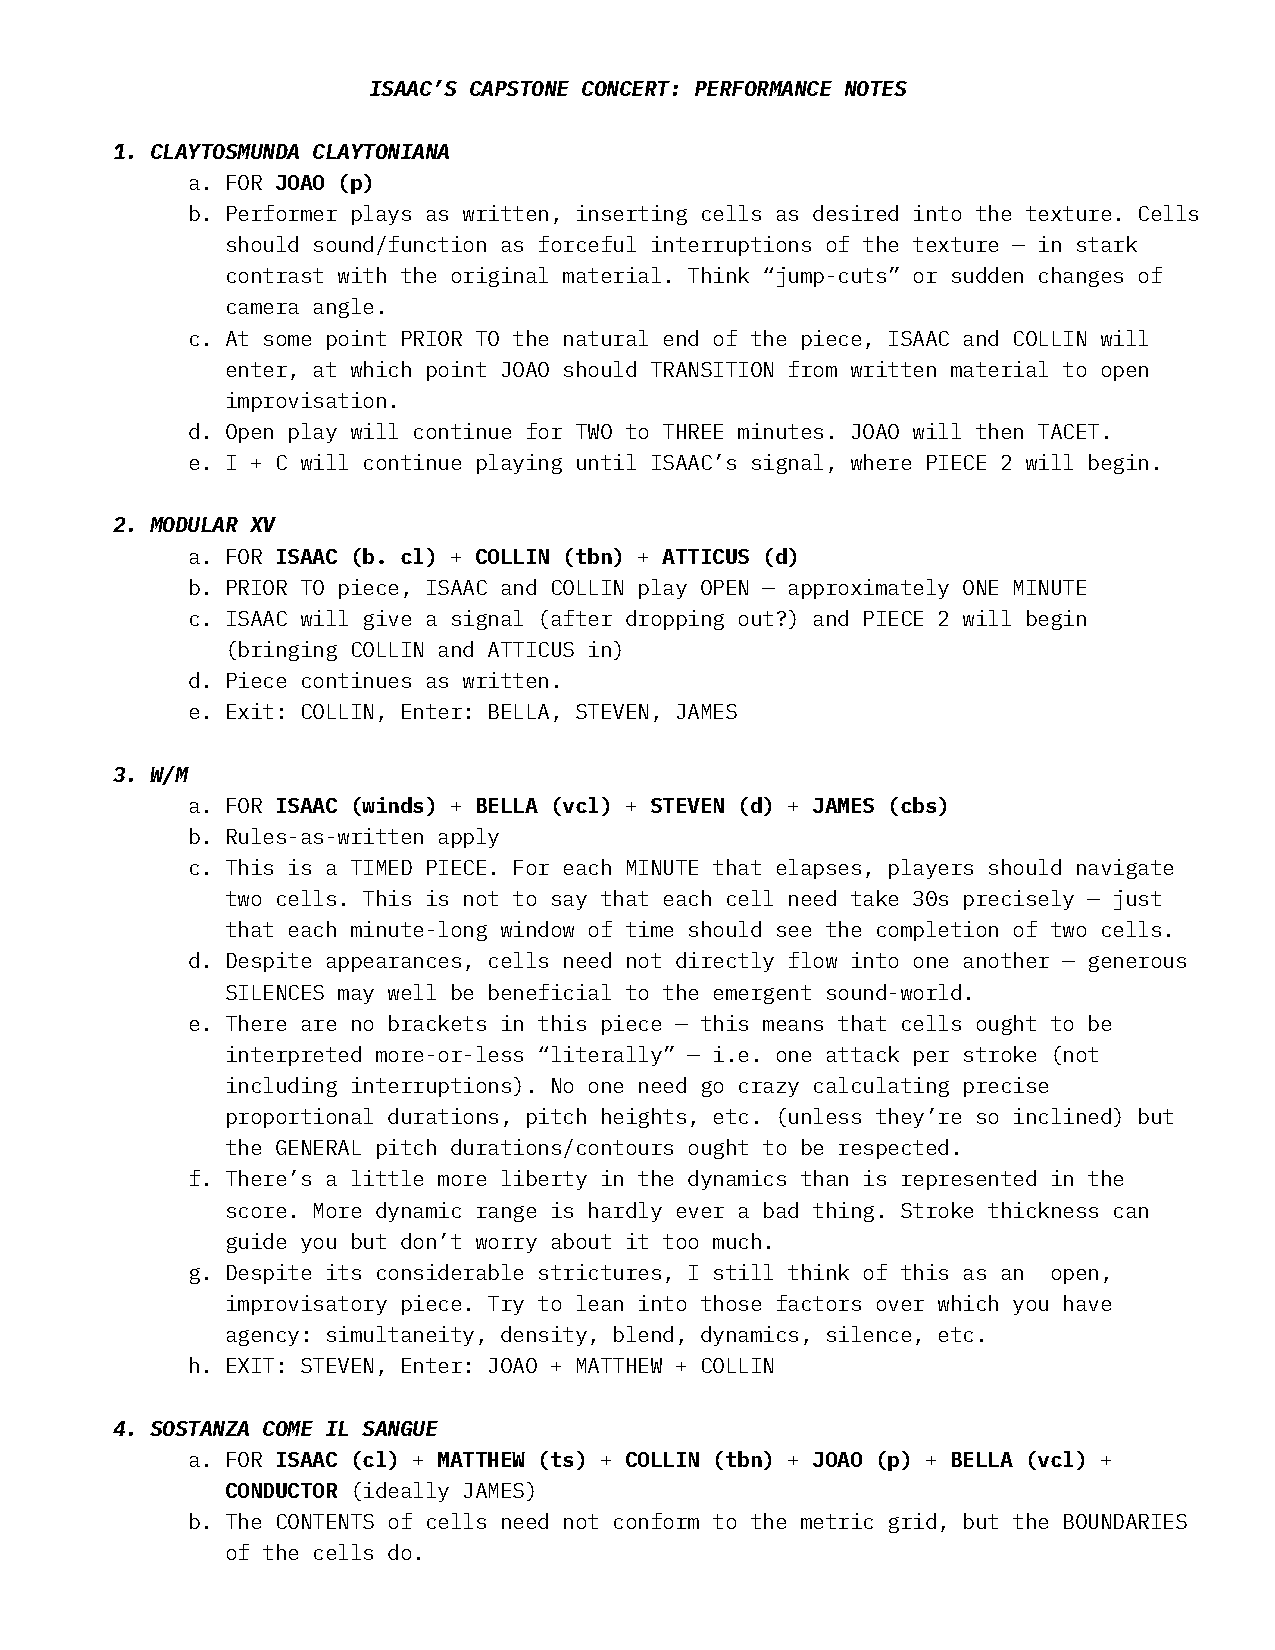
\includepdf[
            pagecommand={\thispagestyle{plain}},
            pages=-,
            frame,
            scale=0.85]{appendix_files/capstone_composition_notes.pdf}
            
    \addtocontents{toc}{\protect\setcounter{tocdepth}{2}}

\chapter{\textit{W/M} (2022)}
    \addtocontents{toc}{\protect\setcounter{tocdepth}{0}}

        \includepdf[
            pagecommand={\thispagestyle{plain}},
            pages={2,1},
            frame,
            angle=270,
            scale=0.85]
            {appendix_files/03WM.pdf}
    
    \addtocontents{toc}{\protect\setcounter{tocdepth}{2}}

\chapter{\textit{Q-Tet} (2023)}
    \addtocontents{toc}{\protect\setcounter{tocdepth}{0}}

        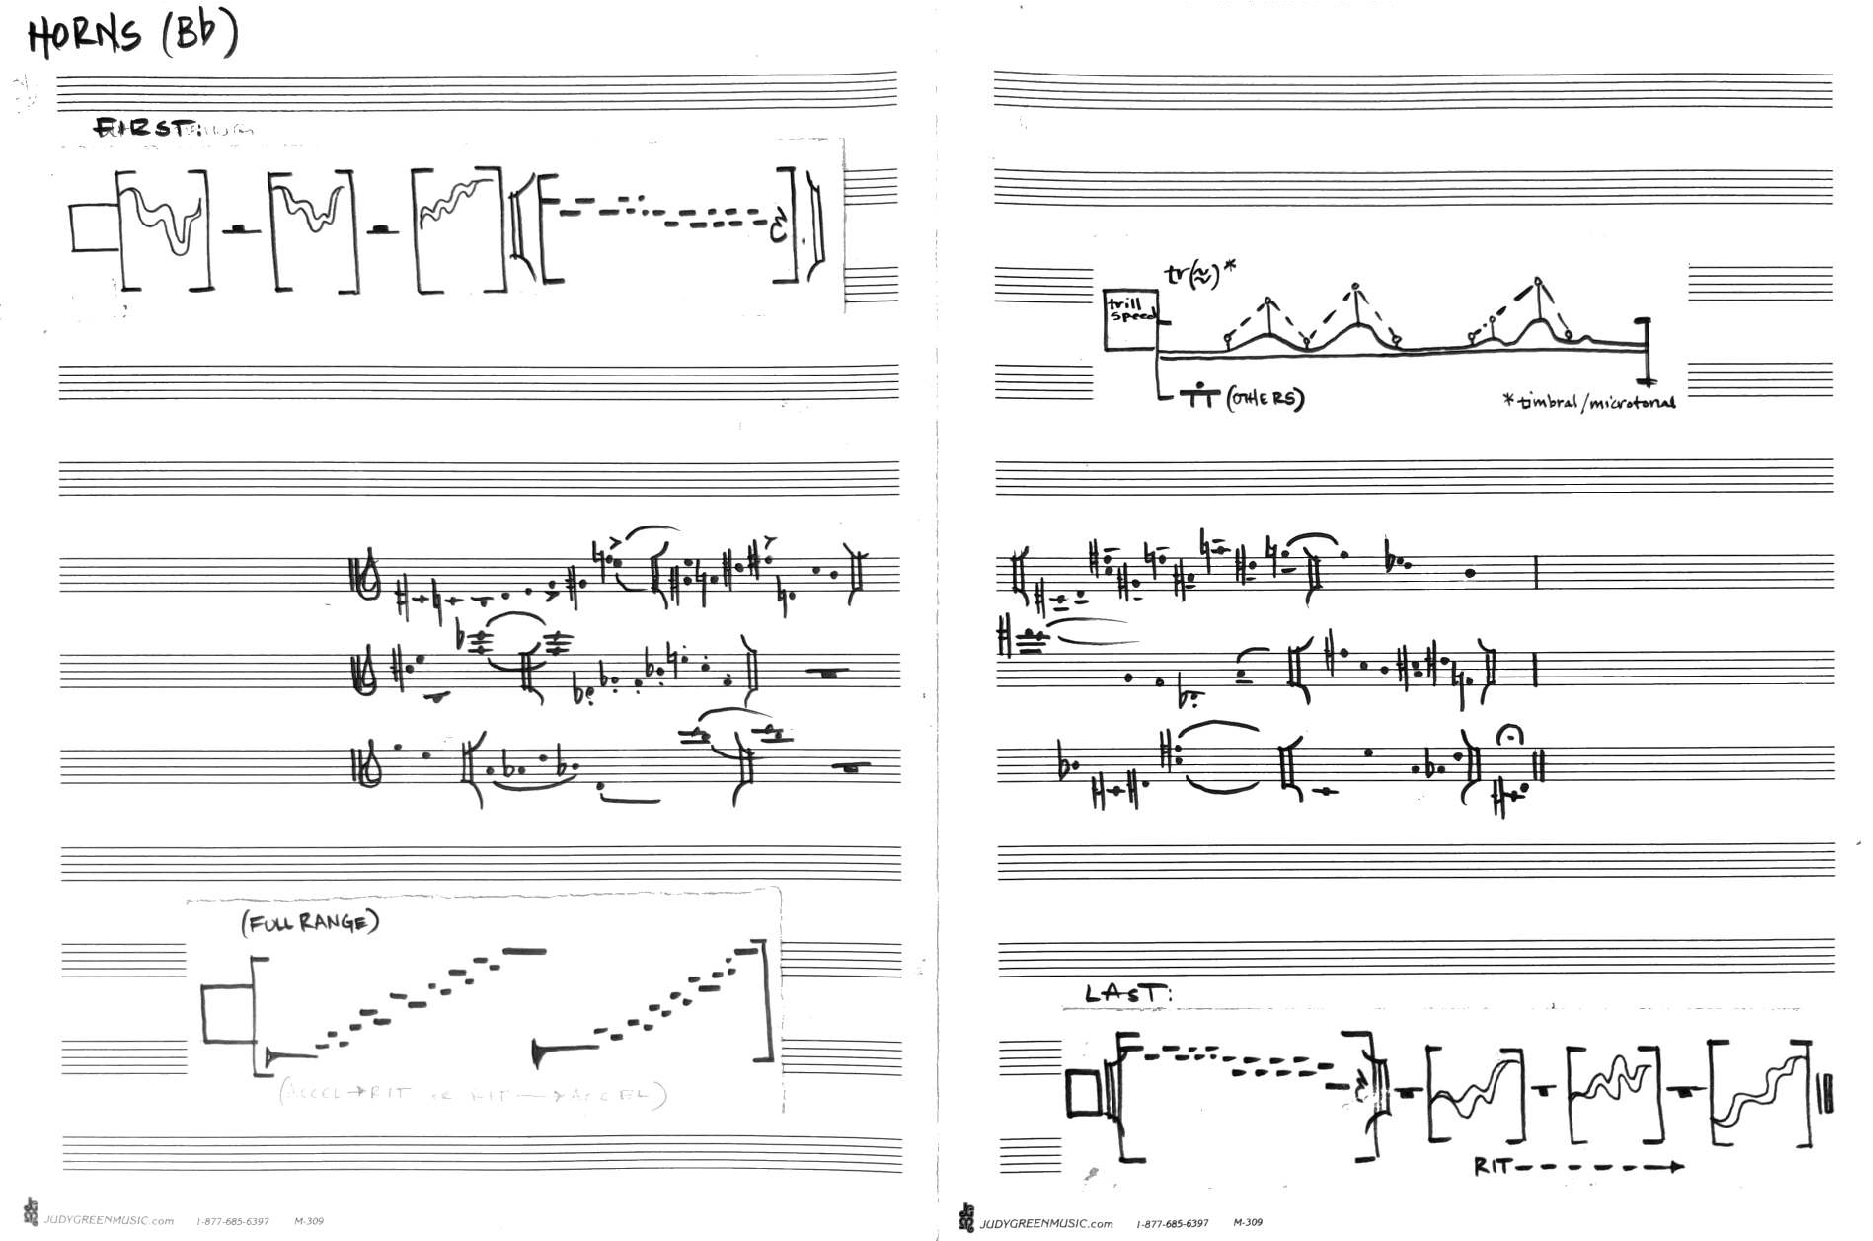
\includepdf[
            pagecommand={\thispagestyle{plain}},
            pages=-,
            frame,
            angle=270,
            scale=0.85]
            {appendix_files/05QTET.pdf}
    
    \addtocontents{toc}{\protect\setcounter{tocdepth}{2}}

\chapter{\textit{Sostanza come il Sangue} (2023)}
    \addtocontents{toc}{\protect\setcounter{tocdepth}{0}}
    
        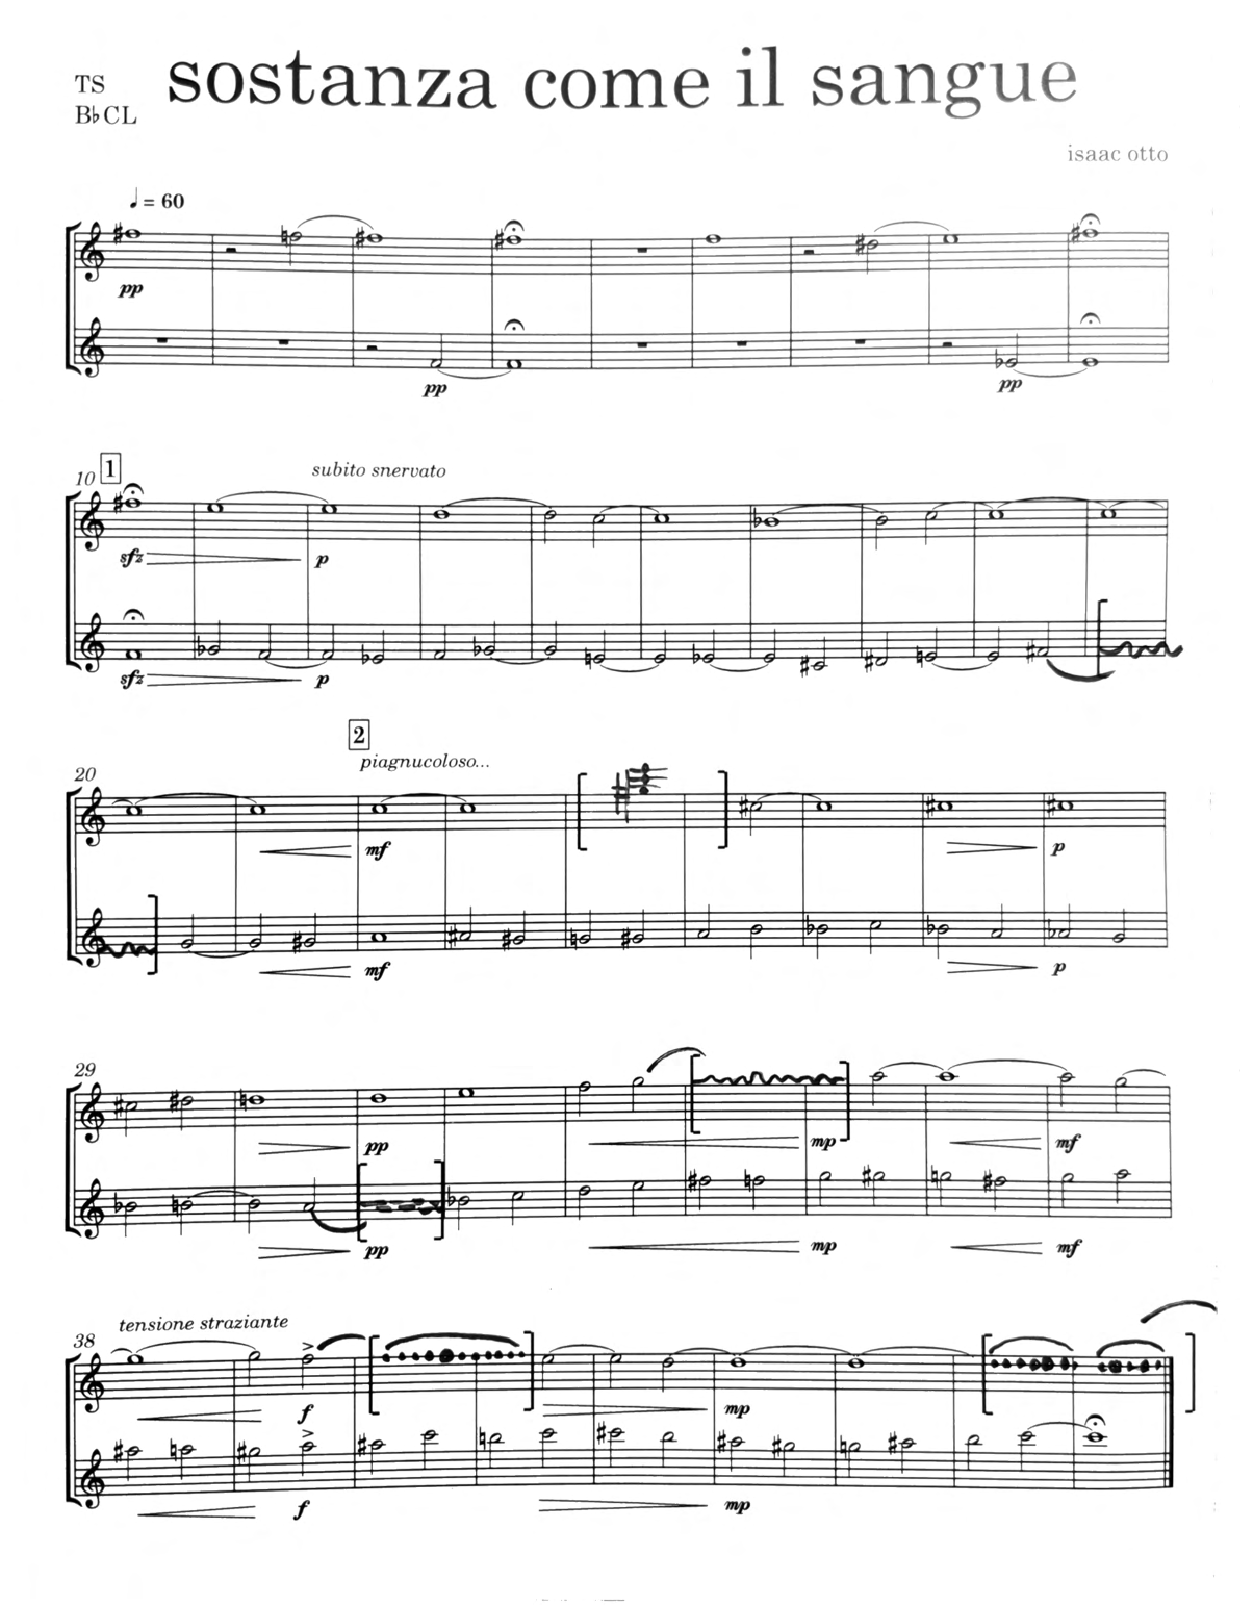
\includepdf[
            pagecommand={\thispagestyle{plain}},
            pages=-,
            nup=1x2,
            frame,
            angle=270,
            scale=0.85]
            {appendix_files/04SOSTANZA.pdf}
    
    \addtocontents{toc}{\protect\setcounter{tocdepth}{2}}

\chapter{\textit{High Structure Carbon Black} (2023)}
    \addtocontents{toc}{\protect\setcounter{tocdepth}{0}}

        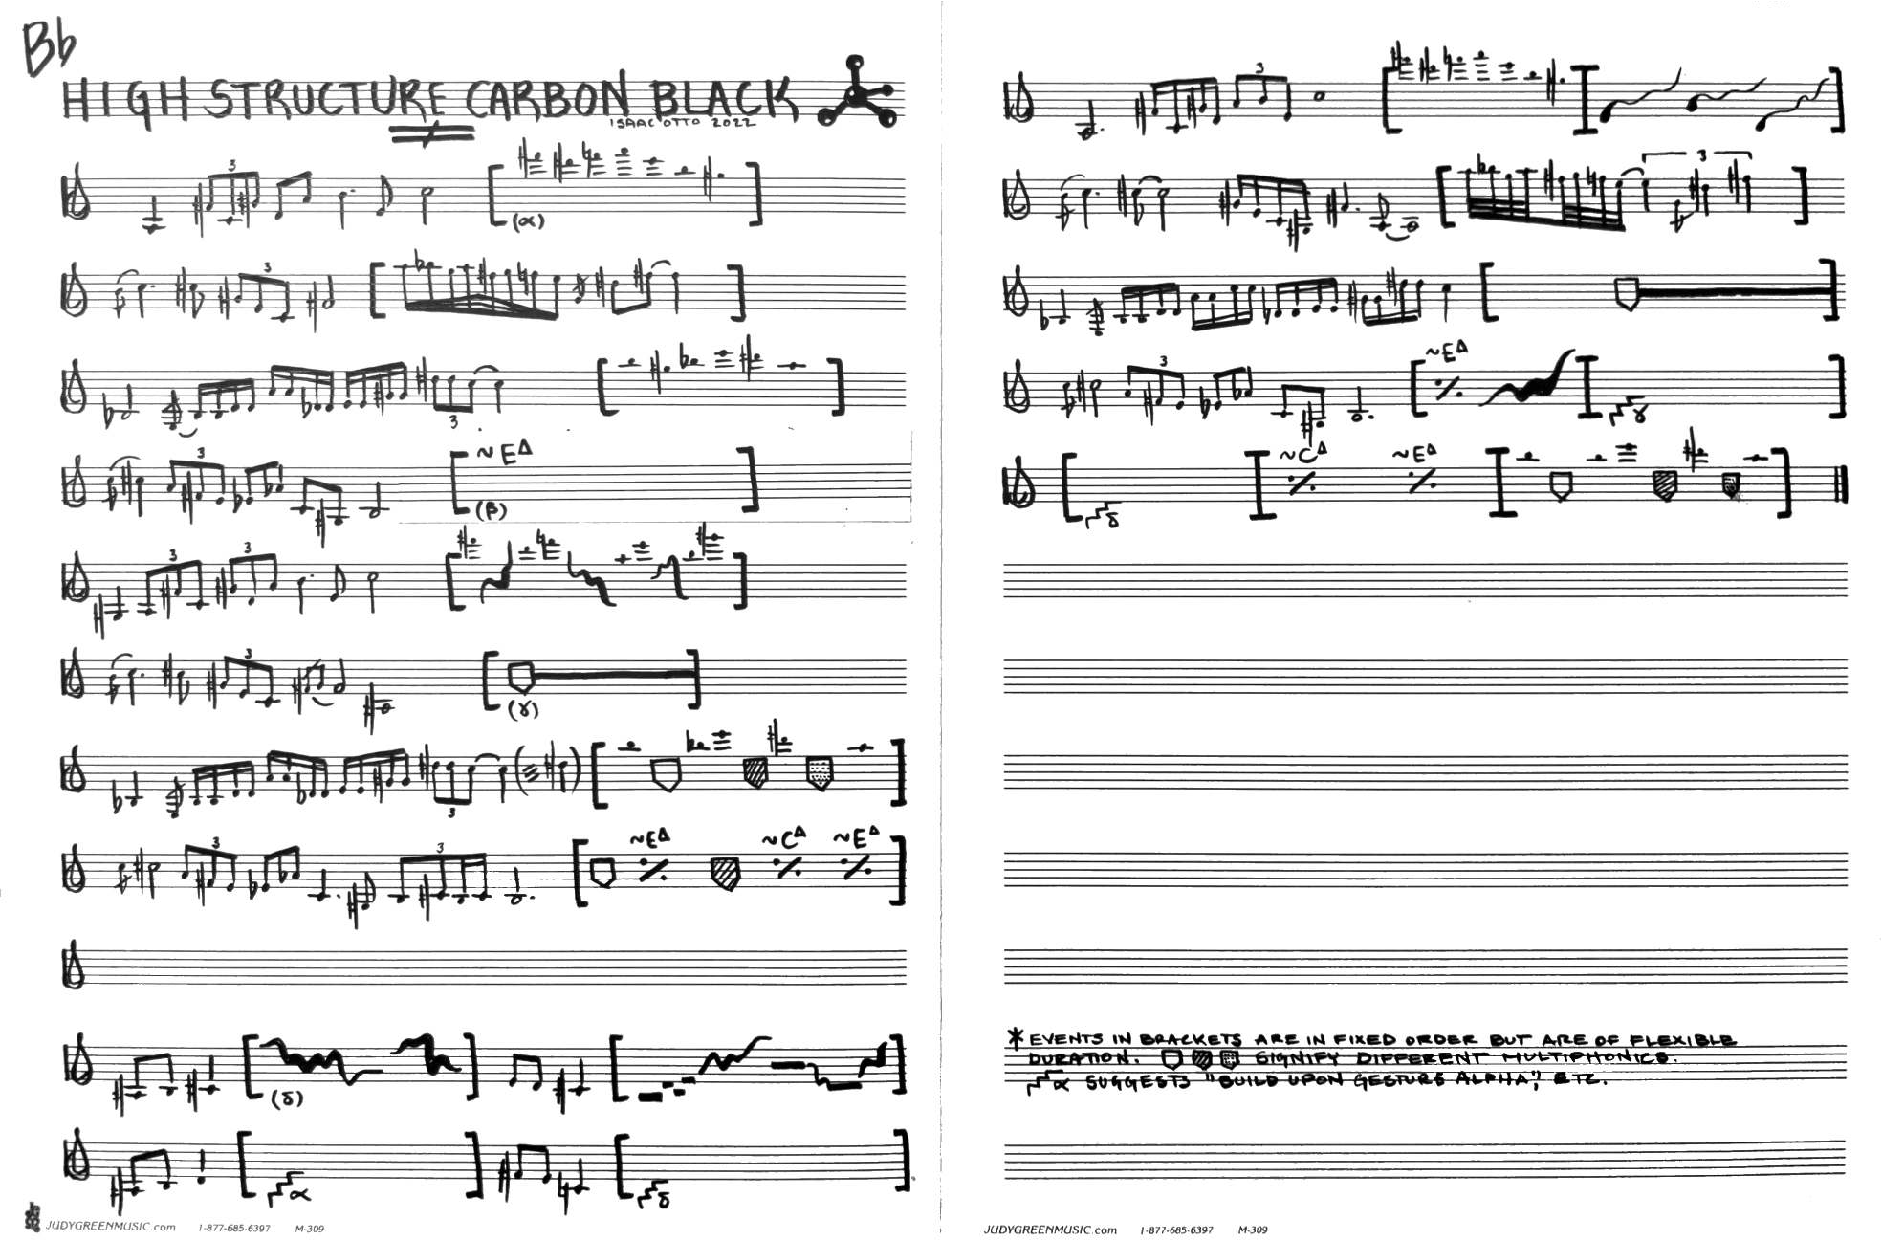
\includepdf[
            pagecommand={\thispagestyle{plain}},
            pages=-,
            frame,
            angle=270,
            scale=0.85]
            {appendix_files/07HSCB.pdf}
    
    \addtocontents{toc}{\protect\setcounter{tocdepth}{2}}

\chapter{\textit{Nemat-Space} (2023)}
    \addtocontents{toc}{\protect\setcounter{tocdepth}{0}}

        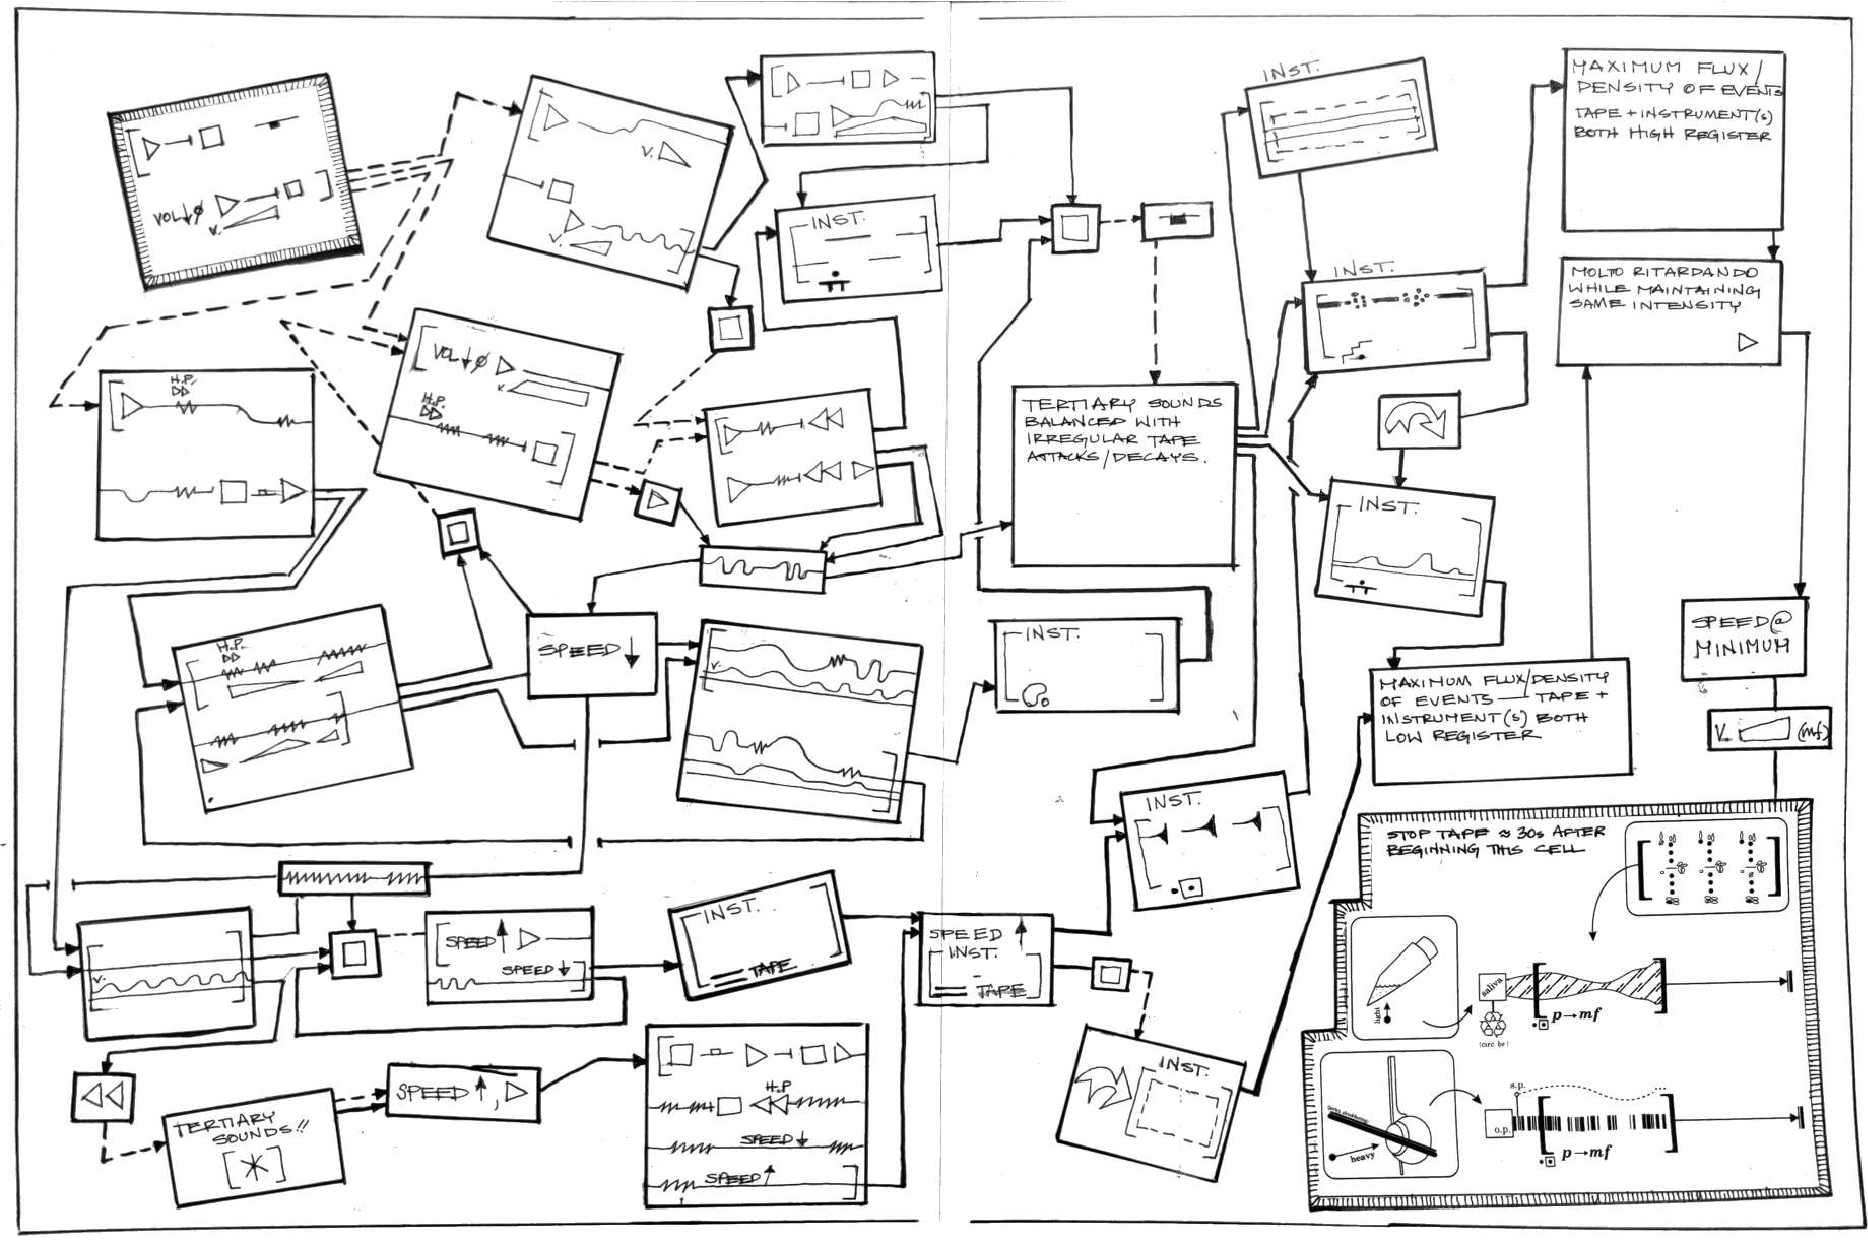
\includepdf[
            pagecommand={\thispagestyle{plain}},
            pages=-,
            frame,
            angle=270,
            scale=0.85]
            {appendix_files/06NEMATSPACE.pdf}
    
    \addtocontents{toc}{\protect\setcounter{tocdepth}{2}}

%%% Local Variables: ***
%%% mode: latex ***
%%% TeX-master: "thesis.tex" ***
%%% End: ***
